\documentclass[../../time_series_notes.tex]{subfiles}
\begin{document}
%%%%%%%%%%%%%%%%%%%%%%%%%%%%%%
\section{Walkthrough Example}
In this section, we look at fitting a SARIMA model on the USAccDeaths data set which contains the number of total accidental deaths in USA at a monthly levels. The data set has two columns, the year-month column and the deaths total. Complete code is avaialable in file time\_series\_python.py
\begin{itemize}
    \item We begin by plotting the data \ref{fig:arima_ex_2}
    \item We notice that there is a seasonality component involved. Also, the mean of the series is not 0. Let's start by doing a seasonal difference first \ref{fig:arima_ex_2}.
    \item There is still some trend. A simple $1^{st}$ order difference should remove this trend. \ref{fig:arima_ex_3}
    \item This is an almost stationary series. We continue the analysis by preparing the ACF and PACF \ref{fig:arima_ex_5}.
    \item From the ACF plot, there are only two peaks that are separated by a lag of 12. Hence, the non-seasonal MA is $\leq 1$ and seasonal MA $\leq 1$.
    \item From the PACF plot, there are two nearby peaks at lag 1 and 2, and there is one more peak at lag 12. Hence, the non-seasonal AR is $\leq 2$ and seasonal AR $\leq 1$.
    \item We chose the model $(p,d,q,P,D,Q) = (0,1,1,0,1,1)$ after checking the AIC for various combinations and following the rule of thumb that $p+d+q+P+D+Q \leq 6$. Results summary in \ref{fig:arima_ex_6}.
    \item Our model equation becomes
    \begin{align*}
        (1-B)(1-B^{12})X_{t} &= (1 - 0.4303B)(1 - 0.5527B^{12})Z_{t}\\
        Z_{t} &\sim \mathcal{N}(0, 99350)
    \end{align*}
    and model summary is given in \ref{fig:arima_ex_6}
    \item We check the QQ plot to confirm that the residuals are indeed normally distributed \ref{fig:arima_ex_7}. We also check for any correlations between the residuals \ref{fig:arima_ex_9}.
    \item Barring the noise, no such significant correlations exist. Ljung Box text on the residuals \ref{fig:arima_ex_9} further confirms this. (High $p-values$ imply that we can accept the null hypothesis which is that the data points are independent)
\end{itemize}

\begin{figure}[h]
    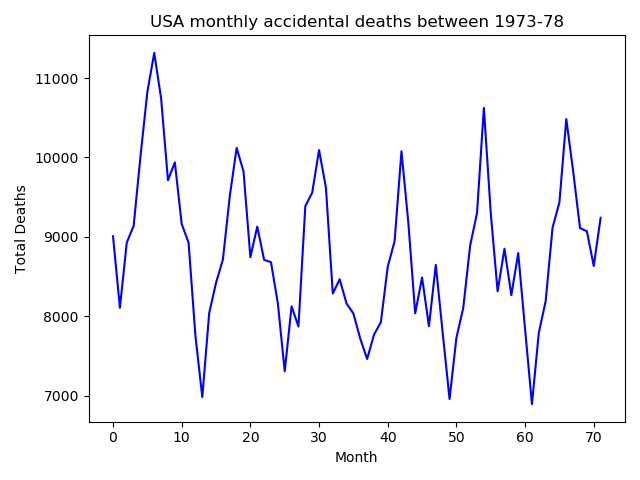
\includegraphics[scale=0.4]{arima_ex_1}
    \centering
    % \caption {Total accidental deaths count between 1973-1978}
    % \label{fig:arima_ex_1} %\ref{fig:arima_ex_1}
    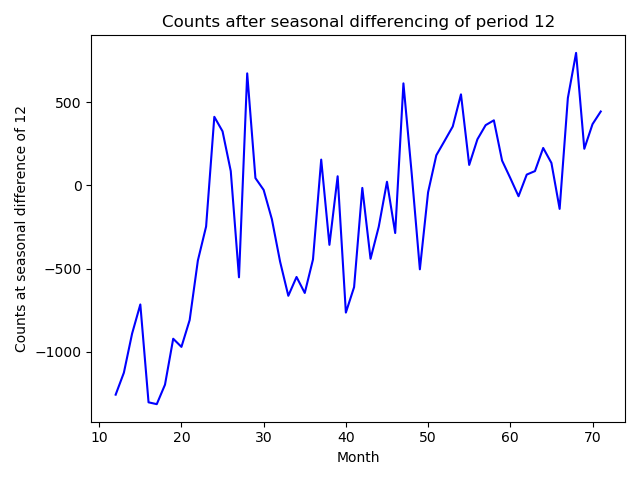
\includegraphics[scale=0.4]{arima_ex_2}
    \centering
    \caption {Left figure is the original time series. Right series is with seasonal differencing (period 12)}
    \label{fig:arima_ex_2} %\ref{fig:arima_ex_2}
\end{figure}

\begin{figure}[h]
    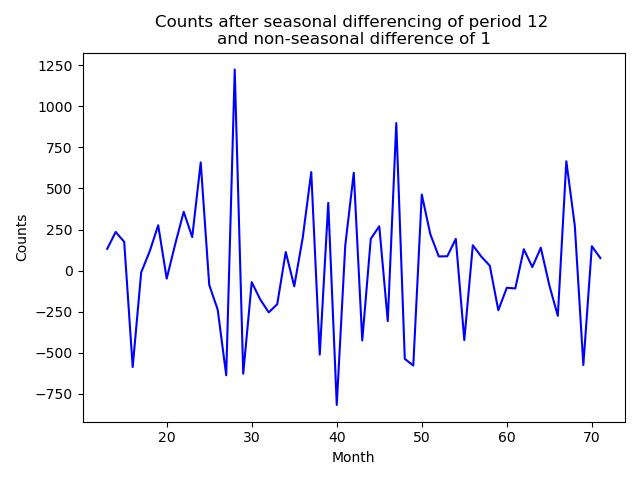
\includegraphics[scale=0.5]{arima_ex_3}
    \centering
    \caption {Time series after non-seasonal difference of 1}
    \label{fig:arima_ex_3} %\ref{fig:arima_ex_3}
\end{figure}

\begin{figure}[h]
    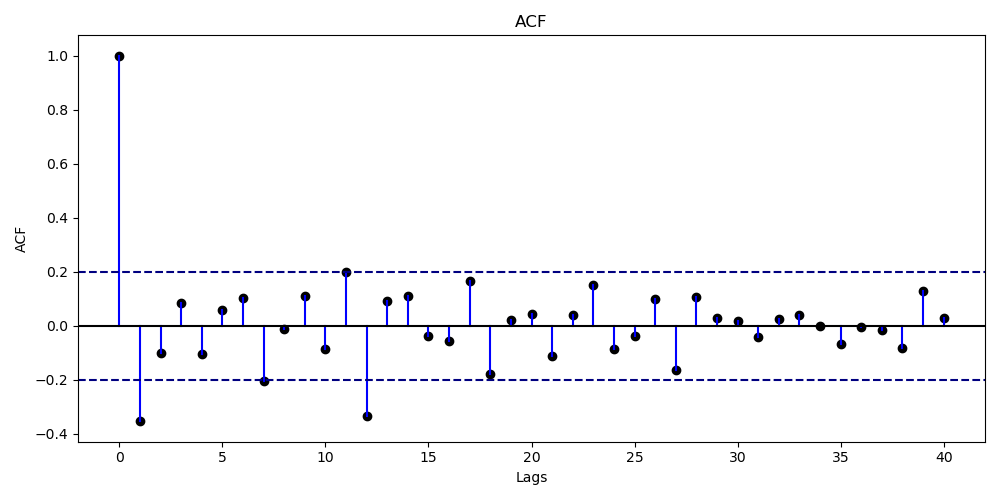
\includegraphics[scale=0.5]{arima_ex_4}
    \centering
    % \caption {Total accidental deaths count between 1973-1978}
    % \label{fig:arima_ex_4} %\ref{fig:arima_ex_4}
    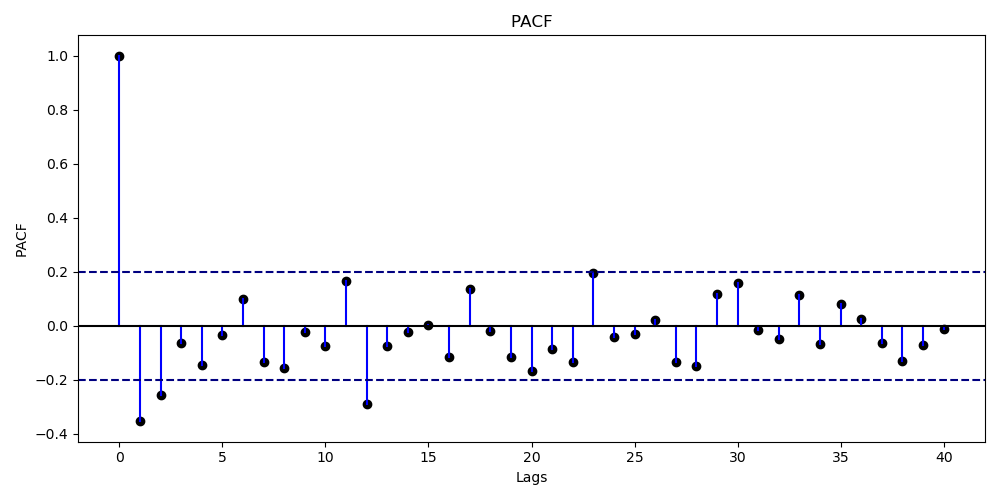
\includegraphics[scale=0.5]{arima_ex_5}
    \centering
    \caption {ACF on top and PACF on bottom.}
    \label{fig:arima_ex_5} %\ref{fig:arima_ex_5}
\end{figure}

\begin{figure}[h]
    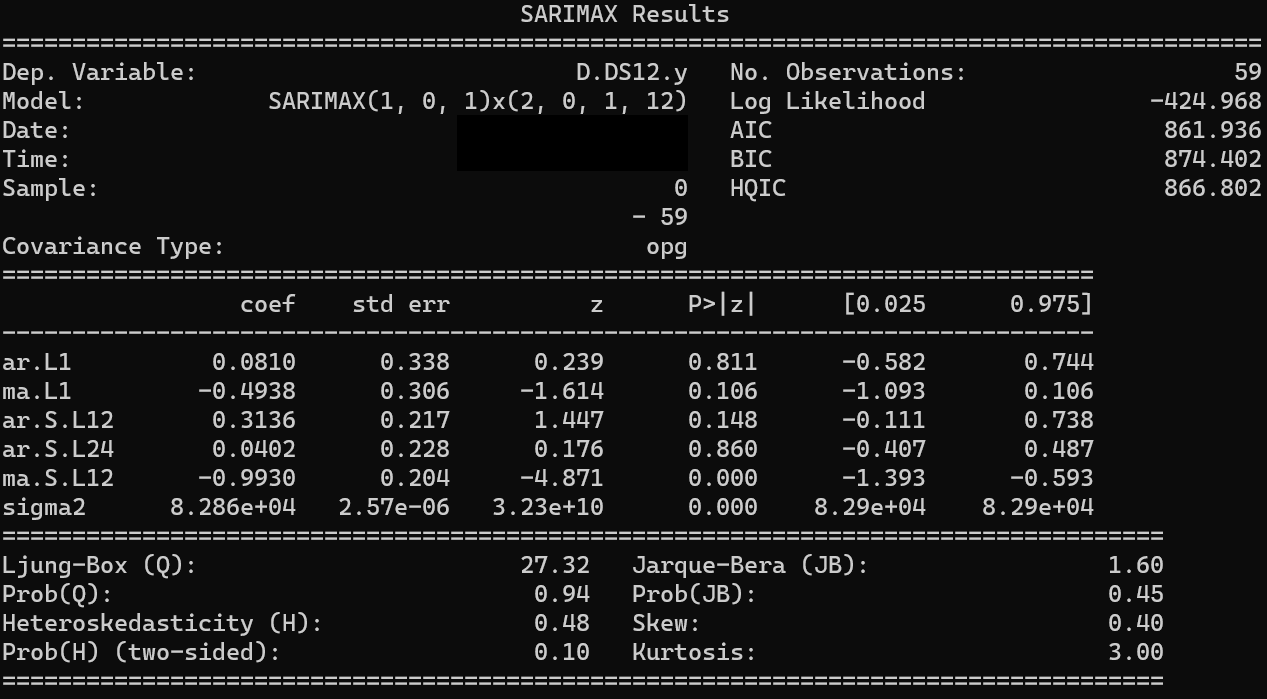
\includegraphics[scale=0.6]{arima_ex_6}
    \centering
    \caption {SARIMAX(0,1,1,0,1,1)12 model summary}
    \label{fig:arima_ex_6} %\ref{fig:arima_ex_6}
\end{figure}

\begin{figure}[h]
    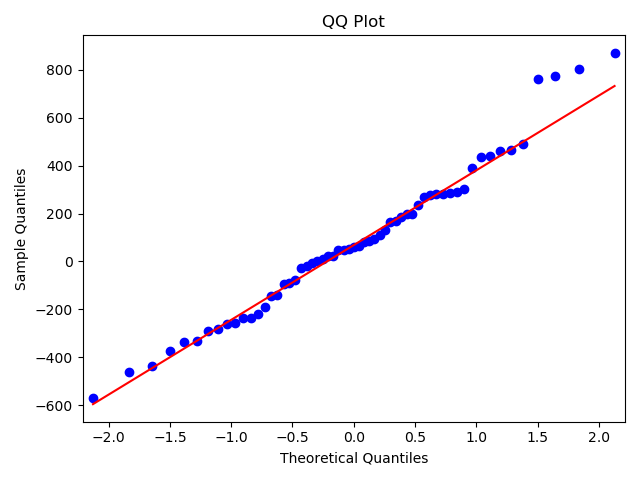
\includegraphics[scale=0.5]{arima_ex_7}
    \centering
    \caption {QQ Plot}
    \label{fig:arima_ex_7} %\ref{fig:arima_ex_7}
\end{figure}

\begin{figure}[h]
    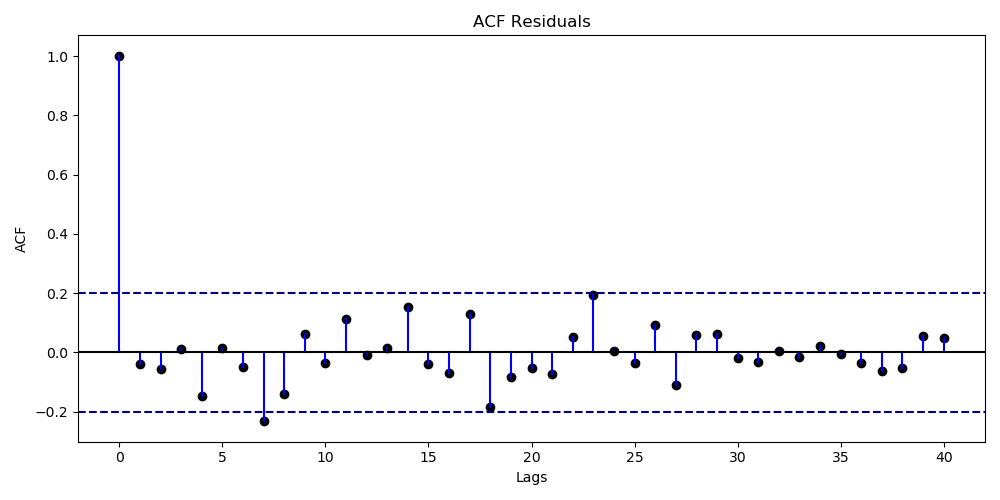
\includegraphics[scale=0.5]{arima_ex_8}
    \centering
    \label{fig:arima_ex_8} %\ref{fig:arima_ex_8}
    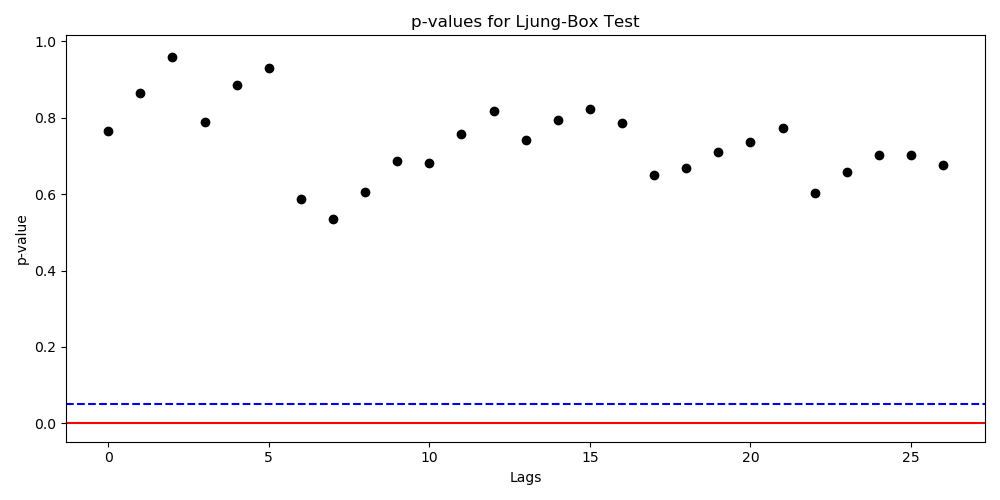
\includegraphics[scale=0.5]{arima_ex_9}
    \centering
    \caption {ACF of residuals on top and $p-values$ from Ljung-Box test on bottom. Dotted blue line is 0.05 significance level.}
    \label{fig:arima_ex_9} %\ref{fig:arima_ex_9}
\end{figure}
\end{document}